
\section{Cloudy models of dust charging around OB stars}
\label{sec:cloudy-models-dust}

\begin{figure*}
  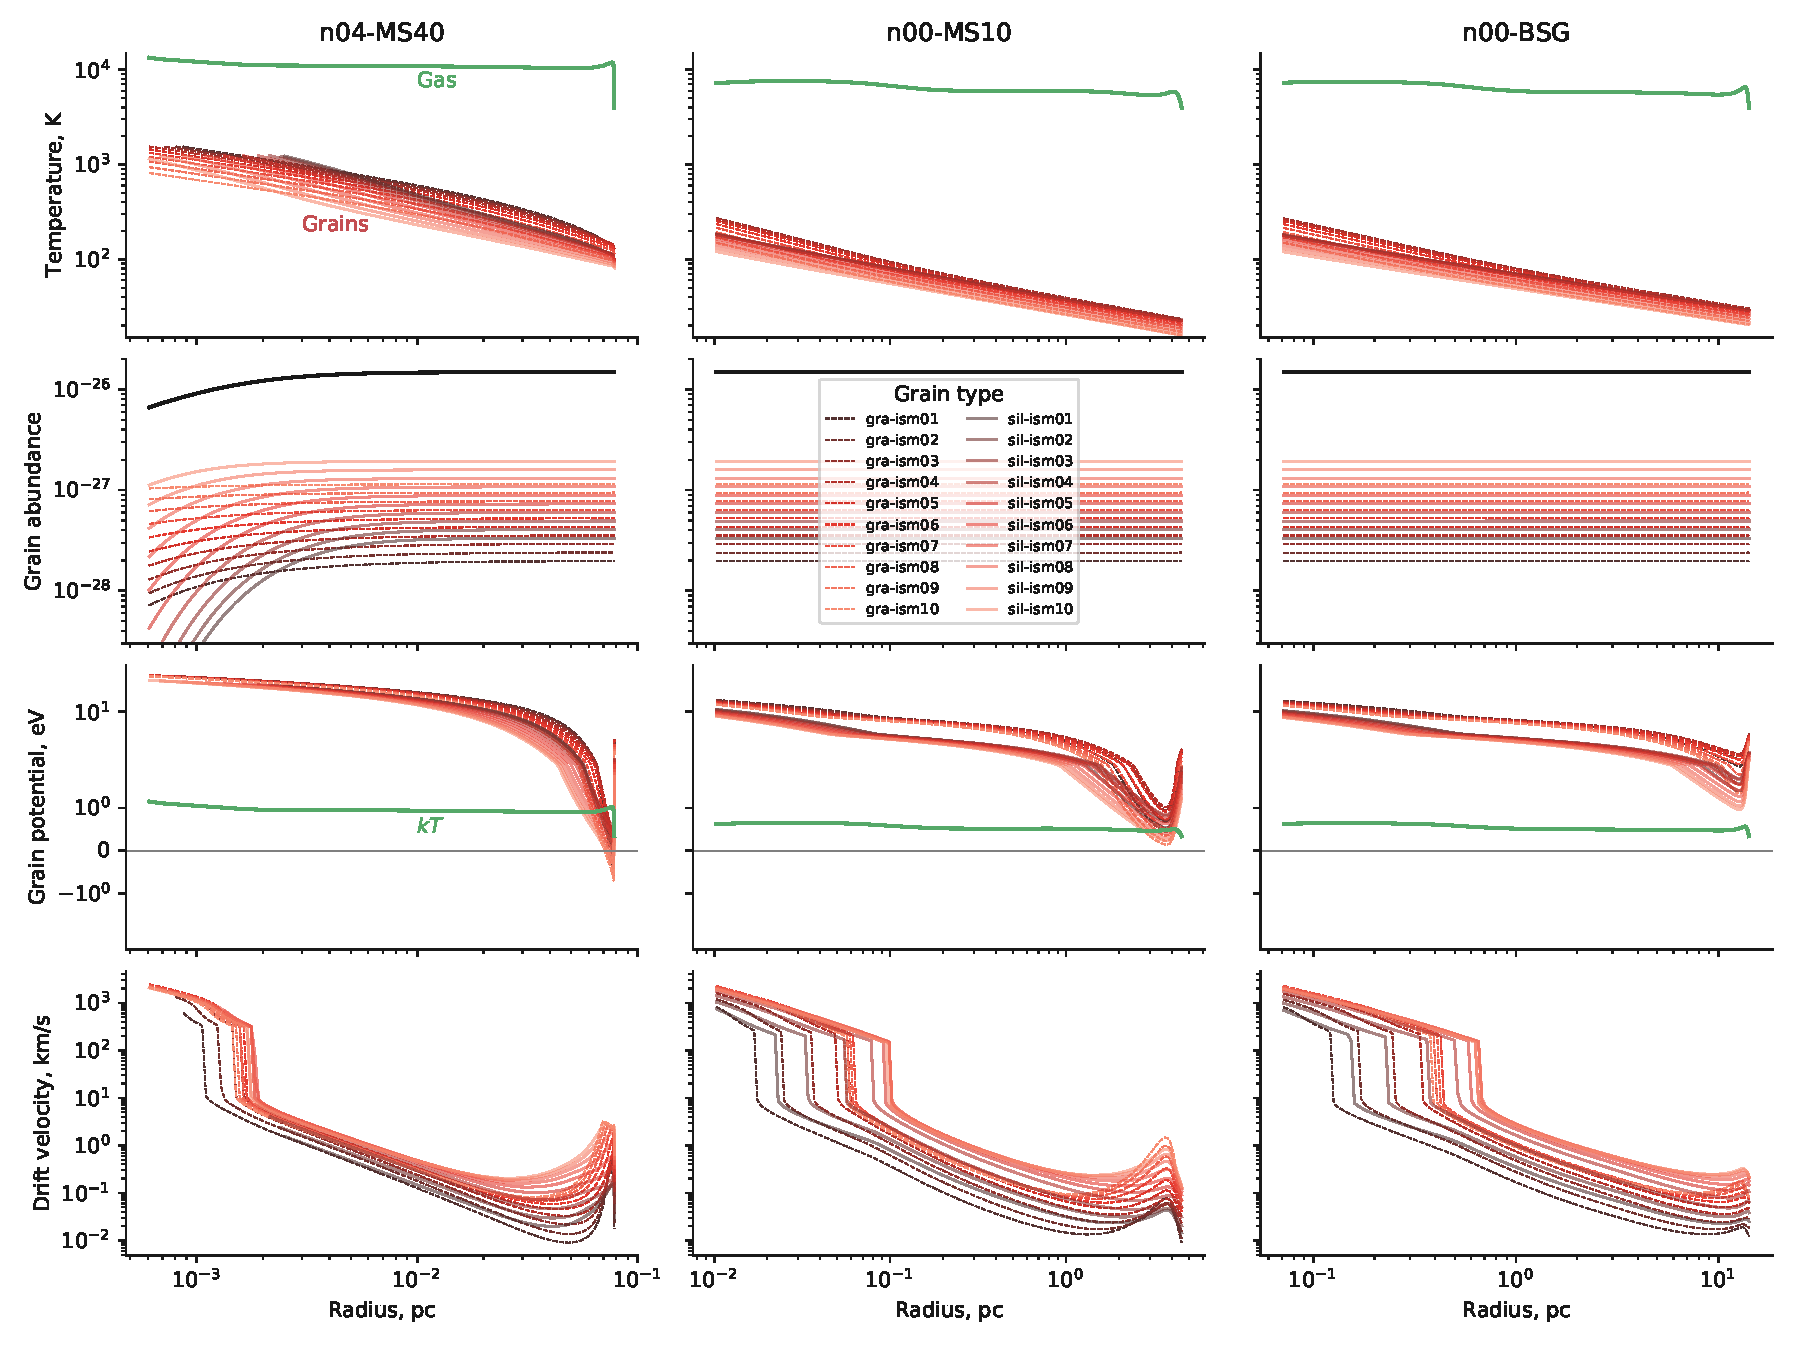
\includegraphics[width=\linewidth]{figs/multi-dustprops}
  \caption{Dust properties as a function of radius from star for three
    selected Cloudy models. (a)~\SI{40}{M_\odot} main-sequence star in
    medium of density \SI{e4}{cm^{-2}}. (b)~\SI{10}{M_\odot} main-sequence
    star in medium of density \SI{1}{cm^{-2}}. (c)~Blue supergiant
    star in medium of density \SI{1}{cm^{-2}}}.
  \label{fig:multi-dustprops}
\end{figure*}

\begin{figure*}
  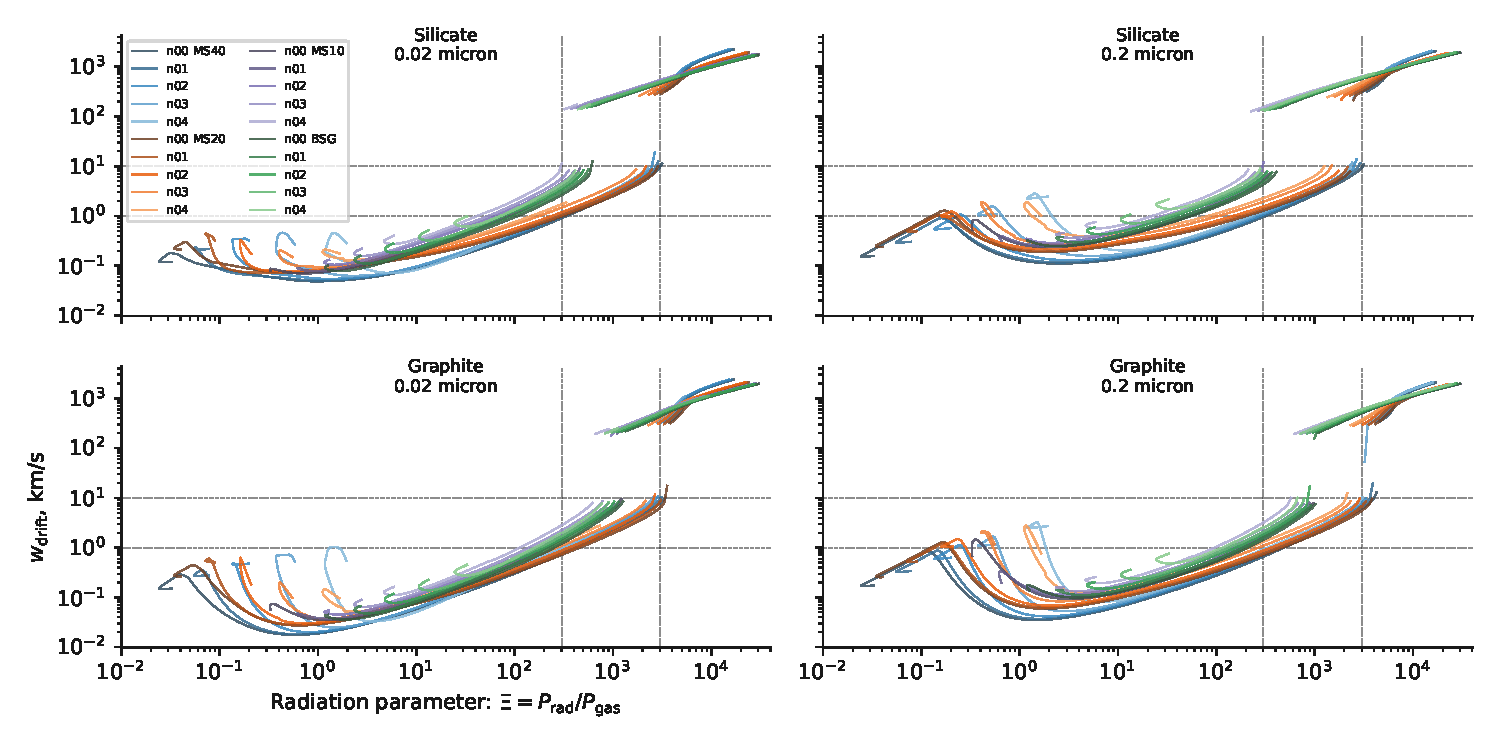
\includegraphics[width=\linewidth]{figs/drift-pratio-4panel}
  \caption{Drift velocity versus radiation parameter \(\Xi_P\). Each line
    represents a model with ambient density and stellar type as
    indicated in the key.}
  \label{fig:drift-gn}
\end{figure*}

\begin{figure}
  \centering
  \includegraphics[width=\linewidth]{figs/phi-versus-xi-annotate}
  \caption{Grain potential versus radiation parameter}
  \label{fig:phi-vs-Xi}
\end{figure}


%%% Local Variables:
%%% mode: latex
%%% TeX-master: "dusty-bow-wave"
%%% End:
